%% LyX 2.3.2 created this file.  For more info, see http://www.lyx.org/.
%% Do not edit unless you really know what you are doing.
\documentclass{article}
\usepackage[utf8]{inputenc}
\usepackage{geometry}
\geometry{verbose,tmargin=2cm,bmargin=2.5cm,lmargin=2.3cm,rmargin=2cm}
\usepackage{graphicx}

\makeatletter
%%%%%%%%%%%%%%%%%%%%%%%%%%%%%% Textclass specific LaTeX commands.
\newcommand{\lyxaddress}[1]{
	\par {\raggedright #1
	\vspace{1.4em}
	\noindent\par}
}

%%%%%%%%%%%%%%%%%%%%%%%%%%%%%% User specified LaTeX commands.
\usepackage{lipsum}
\usepackage{xr}
\externaldocument{Paper_req-550_SM_V0.6.1}
\usepackage{lineno}
\usepackage[strings]{underscore}

\makeatother

\begin{document}
\title{Empowering the crowd: Feasible strategies \\
 to minimize the spread of COVID-19 \\
 in high-density informal settlements}
\author{Alberto Pascual-García$^{(1,*)}$, Jordan Klein$^{(2)}$, Jennifer
Villers$^{(3,\land)}$, \\
 Eduard Campillo-Funollet$^{(4,\wedge)}$, Chamsy Sarkis$^{(5)}$}

\maketitle
\medskip{}


\lyxaddress{}

\lyxaddress{\begin{center}
(1) Institute of Integrative Biology. ETH-Zürich. Zürich, Switzerland.
\\
 (2) Office of Population Research. Princeton University. Princeton,
NJ, USA. \\
 (3) Princeton Environmental Institute. Princeton University. Princeton,
NJ, USA. \\
 (4) Genome Damage and Stability Centre. University of Sussex. Brighton,
United Kingdom. \\
 (5) Pax Syriana Foundation. Valetta, Malta. \\
 ($\land$) Equal contribution. \\
 ({*}) correspondence: alberto.pascual@env.ethz.ch 
\par\end{center}}
\begin{abstract}
More than 1 billion people live in informal settlements worldwide,
where precarious living conditions pose unique challenges to managing
a COVID-19 outbreak. Taking Northwest Syria as a case-study, we simulated
an outbreak in high-density informal Internally Displaced Persons
(IDP) camps using a stochastic Susceptible-Exposed-Infectious-Recovered
model. Expanding on previous studies, taking social conditions and
population health/structure into account, we modeled several interventions
feasible in these settings: moderate self-distancing, self-isolation
of symptomatic cases, and protection of the most vulnerable in “safety
zones”. We considered complementary measures to these interventions
that can be implemented autonomously by these communities, such as
buffer zones, daily health-checks, and carers for isolated individuals,
quantifying their impact on the micro-dynamics of disease transmission.
All interventions significantly reduce outbreak probability and mortality.
Self-distancing reduces mortality by up to 35\% if contacts are reduced
by 50\%. A similar reduction in mortality can be achieved by providing
1 self-isolation tent per 200 people. Protecting the most vulnerable
in a safety zone has synergistic effects with the other interventions
and reduces mortality in the most vulnerable population. Our model
predicts that a combination of all simulated interventions may reduce
mortality by as much as 80\% and delay an outbreak’s peak by more
than three months. Our results highlight the potential for non-medical
interventions to mitigate the effects of the pandemic. Similar measures
may be applicable to controlling COVID-19 in other informal settlements,
particularly IDP camps in conflict regions, around the world. 
\end{abstract}
\newpage{}

\section*{Introduction}

The COVID-19 pandemic is intensifying in the developing world \cite{Guardian1M}.
In Africa, SARS-CoV-2 has been spreading from urban areas to informal
settlements \cite{WHO_AfricaMarks6months}. With more than 1 billion
people living in informal settlements worldwide, urgent action is
needed to contain the virus in these settings, a task which necessarily
involves the engagement of the communities living in them \cite{wilkinson_local_2020}.

The need for action is even more pressing in regions immersed in protracted
armed conflicts, where large portions of their populations have become
displaced. When the displaced population exceeds official resettlement
and refugee camp capacity, Internally Displaced Persons (IDPs) must
live in informal settlements (hereafter named ``camps''). These
regions must contend with the public health challenges resulting from
violence \cite{abbas_migrant_2018}, the deterioration of health-systems
\cite{hill_conflict_2010}, especially of critical care \cite{sahloul_war_2016},
and the breakdown of essential public infrastructure such as water
and sanitation systems \cite{sikder_water_2018}.

This study focuses on the Northwest region of Syria (NWS): a relatively
small geographical area with 4.2 million people, of which 1.15 million
(27.4\%) are IDPs living in camps \cite{Health_directorate}. The
health status of households in camps in NWS is poor; 24\% have a member
with a chronic disease, of whom 41\% have no access to medicines \cite{noauthor_syria_nodate}.
As in other conflict regions, the political instability in NWS hinders
coordinated public health actions, and the ongoing movements of IDPs
create ample opportunity for infectious disease transmission, while
making contact tracing interventions infeasible.

To investigate feasible COVID-19 prevention interventions in the camps,
we considered a Susceptible-Exposed-Infectious-Recovered model similar
to the one presented in \cite{gatto_spread_2020}, in which the camps'
populations are divided into classes reflecting their estimated age-structures
and comorbidity prevalence. We use this model to propose various interventions
aimed at reducing the number of contacts within and between population
classes in general, and with symptomatic individuals in particular.
We paid special attention to how the living conditions in informal
camps inform the assumptions underlying our proposed interventions.
We modeled interventions previously proposed for African cities \cite{vanzandvoort2020},
such as self-distancing, isolation of symptomatic individuals and
the creation of a 'safety zone' in which more vulnerable members of
the population are protected from exposure to the virus.

Building upon the approach used to model the impact of these interventions
in African cities, our model includes a parameterization of the contacts
each individual has per day \cite{vanzandvoort2020}. We further elaborate
upon this approach by making a more explicit representation of contacts
and other parameters in the model. We consider the micro-dynamics
of contacts, the time that individuals take to recognize their symptoms
before self-isolating, the effect of having carers to attend to isolated
individuals, and the existence of a buffer zone in which exposed and
protected population classes can interact under certain rules. We
examine a potential worst-case scenario in which there is no access
to any healthcare facility. Since empowering local communities in
conflict regions to understand how to control COVID-19 is possibly
the most (and perhaps only) effective way to minimize its spread,
our models are of utmost importance for informing the implementation
of realistic interventions in these regions.

\section*{Results}

We considered a discrete-time stochastic model, simulating a viral
outbreak in a single camp over a 12-month period (see Materials and
Methods). In NWS, there are 4 active and 2 planed COVID-19 referral
hospitals, with a current capacity of 66 ventilators, 74 ICU beds
and 355 ward beds for 4.2 million people \cite{REACH_syriaOverview,UNOCHA_CCTC_numbers}.
Basic estimation predicted a collapse of health facilities 8 weeks
into an outbreak \cite{hariri_SyriaForecast_2020}. Hence, we considered
a worst-case scenario in which individuals will not have access to
healthcare and assumed that all critical cases (those requiring ICU
care) would die. We simulated two possible scenarios for the fate
of severe cases (those requiring hospitalization but not ICU care):
one in which all cases recover, and another in which all die. In the
absence of interventions, the mean IFR is $\sim$2\% in simulations
where all severe cases requiring hospitalization recover (see Supplementary
Fig. \ref{fig:Suppl_DvsR}), and $\sim$11\% in simulations where
all severe cases die. We consider the latter scenario to evaluate
the effect of non-medical preventive interventions. In this scenario,
the probability of observing an outbreak is close to 0.85, in which
$\sim$10\% of the camp dies, the number of symptomatic cases peaks
after 55 days and $\sim$84\% of the population recovers.

\begin{figure*}
\includegraphics[width=1\textwidth]{figures/Fig1}

\caption{\textbf{\label{fig:Interventions}Diagram of interventions.}}
\end{figure*}


\subsection*{Self-distancing}

The first non-medical intervention that we modeled is a reduction
in the mean number of contacts per individual per day for the whole
camp population (see Fig. \ref{fig:Interventions}-1). Each individual’s
contact rate (see Supplementary Table \ref{tab:PopParams}) is age
group-specific and was estimated from conversations with camp managers
in NWS. Since the mean number of inhabitants per tent in a camp is
5.5 and sanitation facilities are shared \cite{noauthor_syrian_nodate},
we inferred that the number of contacts per day cannot be reduced
by more than 50\%.For a younger adult, this would mean 7.5 contacts
per day.

Our results show that self-distancing has a notable effect on reducing
the probability of an outbreak: a 20\% reduction in daily contacts
is associated with a $\sim$10\% decrease in outbreak probability
(see Fig. \ref{fig:Panel2}A). A greater reduction in daily contacts,
of 50\%, is required to observe a significant decrease in mortality,
of as much as 35\% (see Fig. \ref{fig:Panel2}B). Self-distancing
also significantly extends the time until the peak of the outbreak,
from 55 days when there is no intervention to 110 days when contacts
are reduced by 50\% (see Fig. \ref{fig:Panel2}C). However, the proportion
of the population recovered after 12 months is reduced by $\sim$30\%
(see Supplementary Fig. \ref{fig:Suppl_self}).

\begin{figure*}
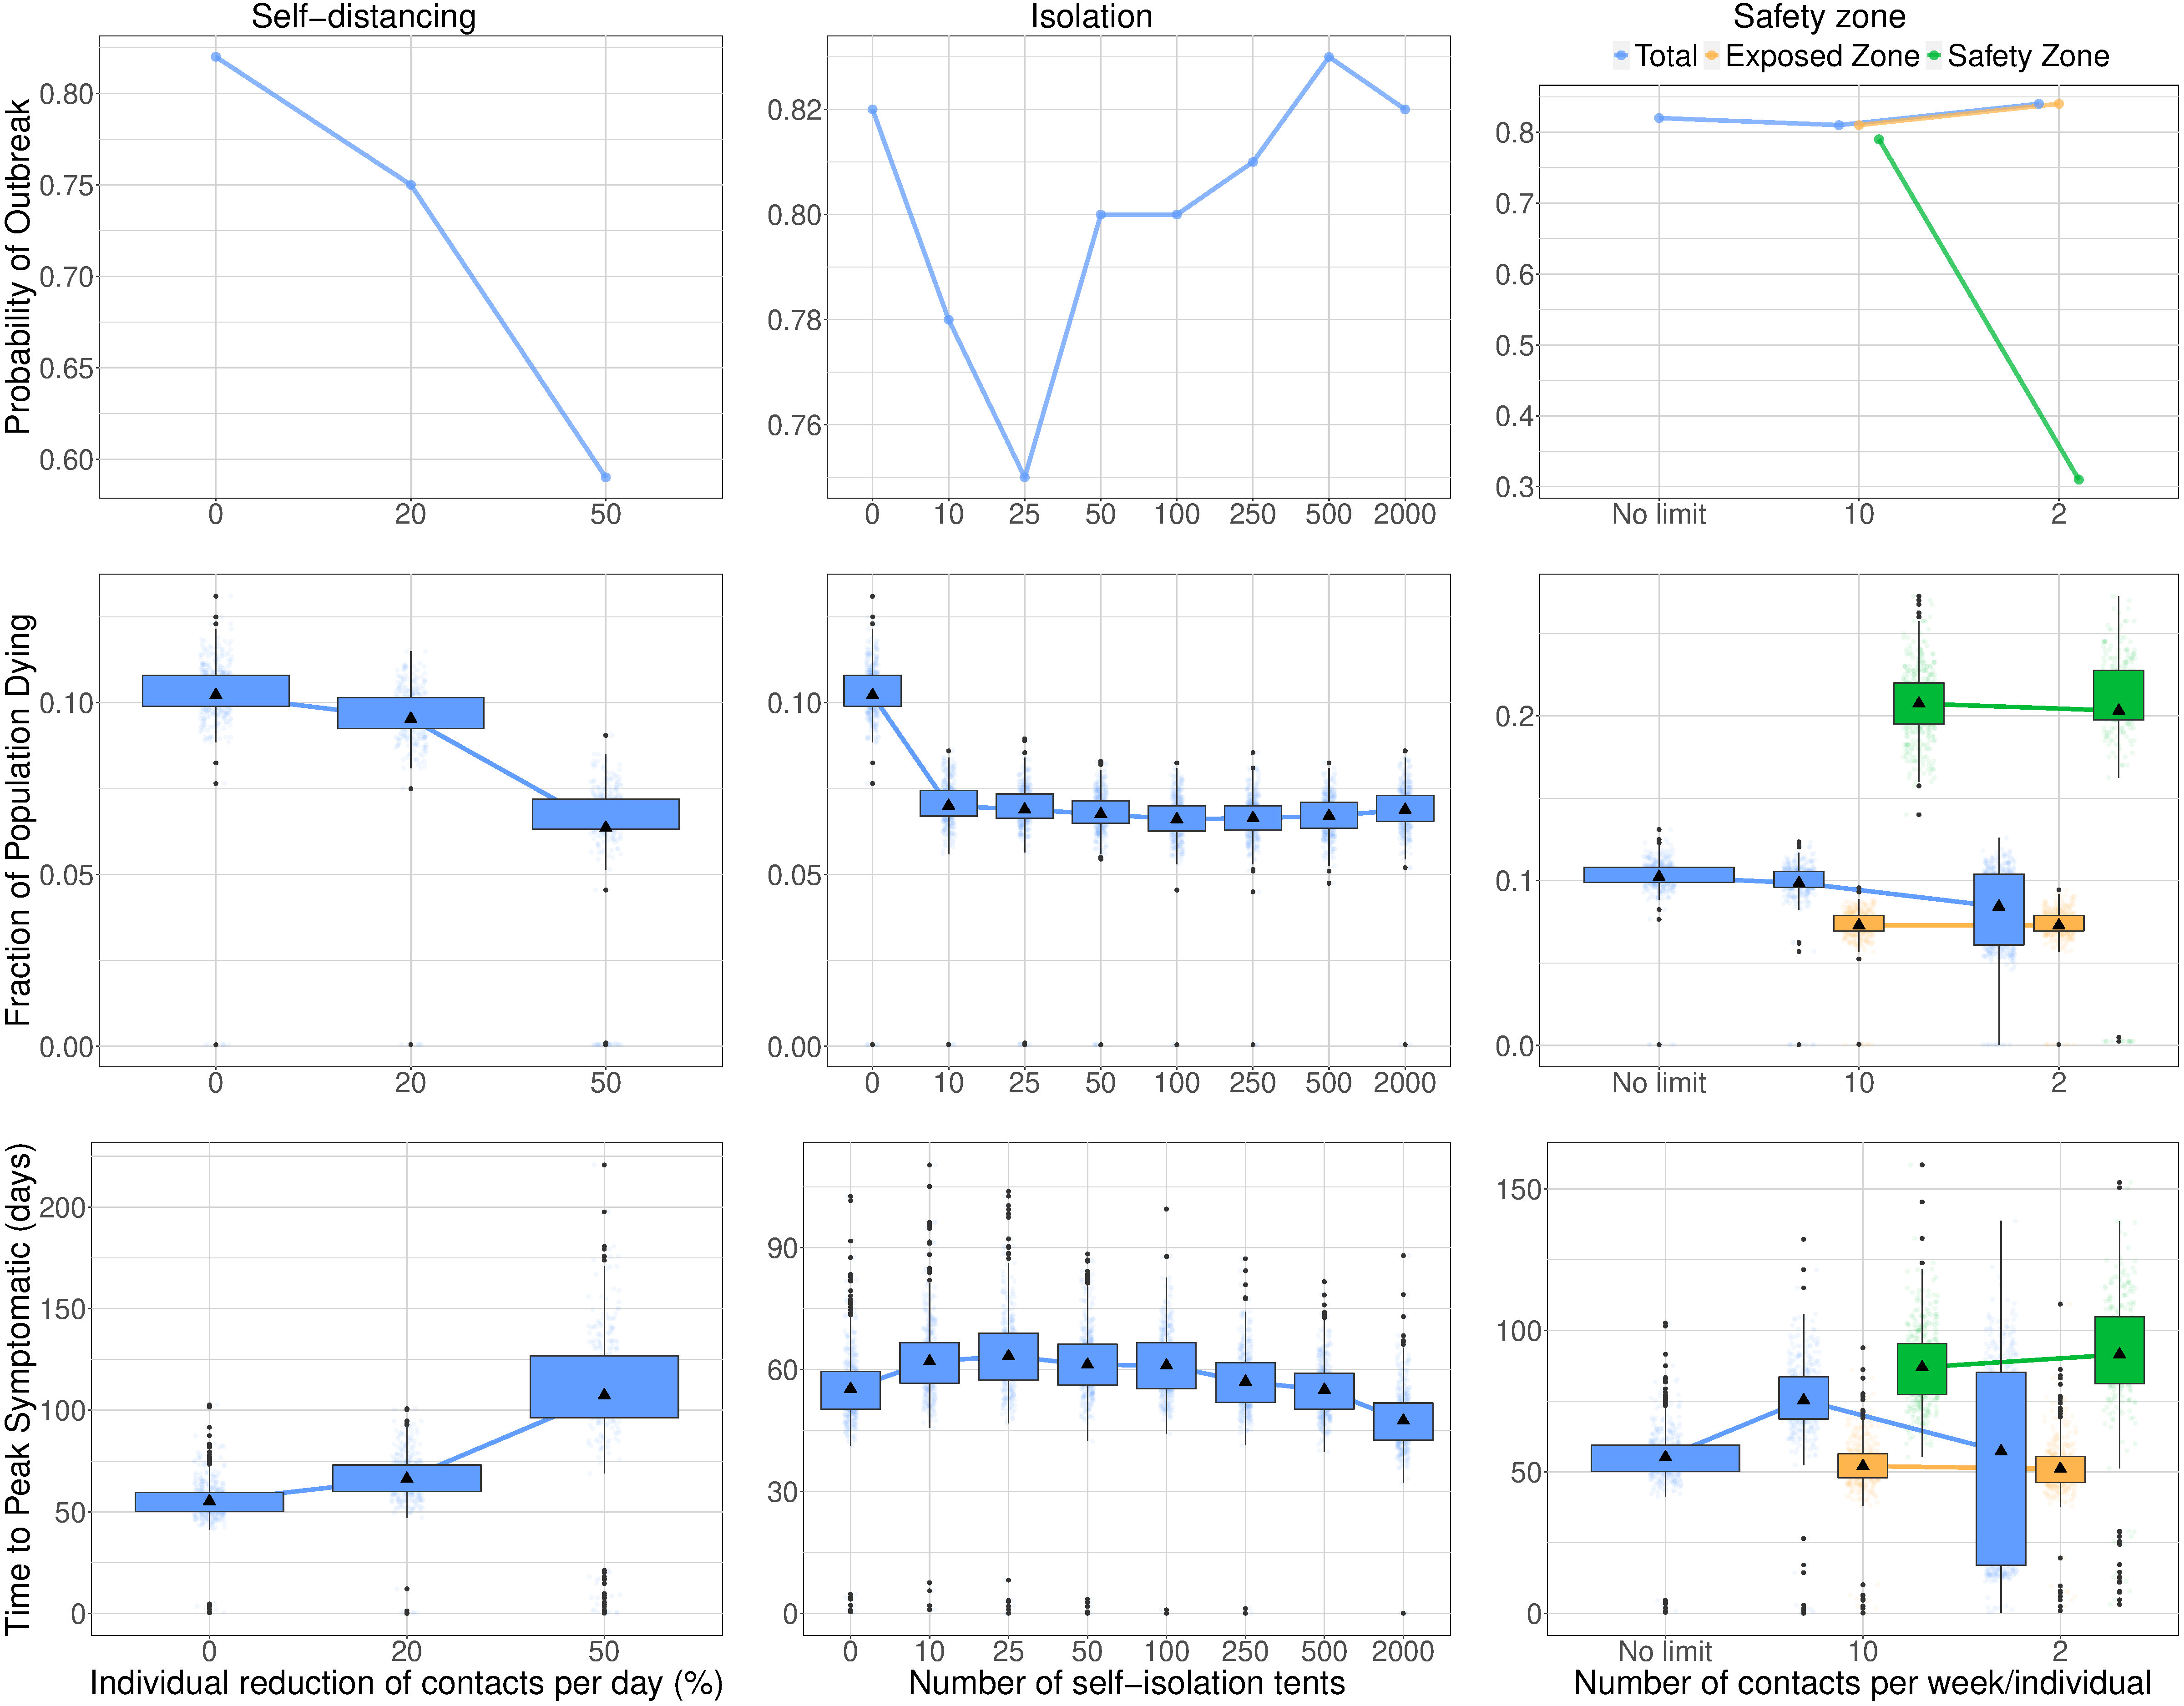
\includegraphics[width=1\textwidth]{figures/Fig2}

\caption{\label{fig:Panel2} \textbf{Effect of interventions on outbreak probability,
fatalities and time until symptomatic cases peak.} A: Self-distancing,
probability of an outbreak. B: Self-distancing, fraction of the population
dying. C: Self-distancing, time until peak symptomatic cases. D: Self-isolation,
probability of an outbreak. E: Self-isolation, fraction of the population
dying. F: Self-isolation, time until peak symptomatic cases. G: Safety
zone, probability of an outbreak. H: Safety zone, fraction of the
population dying. I: Safety zone, time until peak symptomatic cases.
Note that in figures of the safety zone intervention (panels G-I),
the mean of an outcome for the whole population is not the weighted
mean of the exposed and safety zones, since outcomes are computed
considering simulations in which at least one death was observed in
the population class inhabiting the zone. This explains why in panel
I there is a reduction in the mean time until symptomatic cases peak
when moving from 10 to 2 contacts per week for the whole population,
despite there being an increase in the safety zone: in $\sim$35\%
of simulations there is an outbreak in the orange zone but not in
the green zone (panel G).}
\end{figure*}


\subsection*{Self-isolation}

Self-isolation is a challenge in informal settlements, where households
consist of a single (often small) space, water is collected at designated
locations, sanitation facilities are communal and food supplies are
scarce. We considered the possibility of those showing symptoms self-isolating
in individual tents in dedicated parts of the camps. We simulated
this intervention with various numbers of isolation tents per camp,
ranging from 10 to 2000 for a camp of 2000 people (see Fig. \ref{fig:Interventions}-2).
In addition, we modeled the role of carers dedicated to providing
for isolated individuals (see Fig. \ref{fig:Interventions}-2a). Interactions
between carers and isolated individuals were restricted to buffer
zones, which we envisioned as open spaces, with guidelines in place
to limit occupancy to 4 individuals wearing masks, with 2 meters separating
individuals, where the probability of transmission is reduced by 80\%
(see Supplementary Material). In considering one carer per isolated
individual with one contact per day, we do not neglect their probability
of infecting the rest of the camp. We also considered minimum time
intervals for individuals to recognize their symptoms: with means
of 12, 24 and 48 hours (see Fig. \ref{fig:Interventions}-2b).

With only 10 tents for a camp of 2000 people (i.e. 1 tent for every
200 people), self-isolation yields a modest decrease in the probability
of observing an outbreak (see Fig. \ref{fig:Panel2}D), but a stronger
reduction in mortality ($\sim$30\%) (see Fig. \ref{fig:Panel2}E).
Further increasing the number of tents significantly augments this
reduction until there is 1 per every 20 people (Kruskal-Conover post-hoc-test,
p-val$<3\times10^{-5}$). However, mortality begins to slightly increase
again after this threshold. This effect and the increase in the probability
of observing an outbreak are consequences of having one carer per
individual isolated (see Supplementary Material), so when the isolated
(infected) population increases, the number of healthy younger adults
in contact with them increases in tandem. Similarly, we observe a
reduction in IFR when increasing the number of tents up to 1 per every
20 people, and no significant reduction over that number (see Supplementary
Fig. \ref{fig:Suppl_isolation}). Importantly, the potential reductions
in overall fatalities and IFR from self-isolation are realized whether
the time required for individuals to recognize their symptoms is 12h
or 24h on average, but the intervention becomes less effective when
this time increases to 48h (see Supplementary Fig. \ref{fig:Suppl_onset}).

\subsection*{Safety zone}

In this intervention, the camp is divided in two areas: a safety zone,
in which more vulnerable people live (hereby referred to as a “green”
zone following previous studies \cite{vanzandvoort2020}), and an
exposed (“orange”) zone with the remaining population. In our simulations,
the first exposed individual always belongs to the orange zone. The
living conditions within both zones remain the same, so the overall
contact rate does not change unless self-distancing is also implemented.
In practice, reducing the contact rate with individuals living in
a different zone implies an increase in the contact rate with individuals
in the same zone (see Supplementary Material). This allows us to investigate
undesired side-effects of this intervention. Since proposals for partitioning
the population may be received differently across camps, we considered
several scenarios for allocating a camp population to the two zones
(see Fig. \ref{fig:Interventions}-3, Supplementary Table \ref{tab:SafetyScenarios}).
In this section, we consider the scenario in which all older adults,
younger adults with comorbidities and their family members up to 20\%
of the camp population live in the green zone, unless otherwise specified.
Interactions between the two zones are limited to a buffer zone. Individuals
in the green zone cannot leave and thus need to be provided with supplies
by individuals in the orange zone. Delivery of supplies will take
place in the buffer zone. In our simulations, we considered limiting
individuals in the green zone to 10 or 2 contacts with individuals
from the orange zone per week (see Fig. \ref{fig:Interventions}-3a).
Other variations of this intervention we explored include preventing
symptomatic individuals from entering the buffer zone (see Fig. \ref{fig:Interventions}-3b)
and a “lockdown” of the green zone, where the number of weekly contacts
in the buffer zone is reduced by 50\% or 90\% (see Fig. \ref{fig:Interventions}-3c).

Creating a green zone improves the effect of the previous interventions
overall, but with sometimes opposite outcomes in the exposed and protected
populations. For example, the probability of an outbreak sharply decreases
for the protected population, by almost 40\%, if only two contacts
are allowed per week in the buffer zone (see Fig. \ref{fig:Panel2}G).
Notably, most of this reduction is only achieved when health-checks
excluding symptomatic individuals from the buffer zone are in place
(see Supplementary Fig. \ref{fig:Suppl_Tcheck}). On the other hand,
the probability of an outbreak may slightly increase for the exposed
population, a consequence of the relative increase in intra-zone contacts.
Despite this side-effect, by shifting the burden of an outbreak towards
the less vulnerable population in the orange zone, this intervention
not only reduces fatalities among the more vulnerable population in
the green zone (Kruskal-Wallis test, p-val$<10^{-15}$; see Supplementary
Fig. \ref{fig:Suppl_agegroups}), but also reduces the overall IFR
(see Supplementary Fig. \ref{fig:Suppl_safety}) and thus the number
of fatalities globally (see Fig. \ref{fig:Panel2}H). Another important
outcome of this intervention is the notable increase in time until
the number of symptomatic cases peaks for the vulnerable population
(see Fig. \ref{fig:Panel2}I).

Considering different scenarios for allocating people to the green
zone, the lowest probability of an outbreak is achieved when only
older adults or at most older adults and younger adults with comorbidities
move there (see Supplementary Fig. \ref{fig:Suppl_popClass}). Positive
effects of the green zone intervention are even more marked in camps
with smaller populations, for every outcome of interest except time
until symptomatic cases peak (see Supplementary Fig. \ref{fig:Suppl_popSize}).
The incorporation of a lockdown has the greatest effect on reducing
the probability of an outbreak in the green zone, to under 0.10 when
contacts in the buffer zone are reduced by 90\%. While lockdowns show
no positive effect on green zone fatalities in the few instances where
an outbreak does reach there, they decrease IFR and overall fatalities
by further concentrating outbreaks in the less vulnerable population
(see Supplementary Fig. \ref{fig:Suppl_lockdown}).

\subsection*{Evacuation}

The last intervention we simulated is the evacuation of severe cases
(individuals in the hospitalization compartment). Since they require
more intensive care that cannot be delivered while adhering to the
guidelines of a buffer zone, severe cases were assumed to be fully
infectious and not able to self-isolate. Once severe cases are evacuated,
their infectivity is reduced to zero (see Fig. \ref{fig:Interventions}-4).
The fate of severe cases is not altered by this intervention since
we assumed that hospitals are saturated and that evacuees are transferred
to isolation centers instead.

We observe no significant effects when severe cases requiring hospitalization
are evacuated (see Supplementary Fig. \ref{fig:Suppl_evacuation}).
Although the period between developing more severe symptoms and dying
is relatively long ($\sim$10 days), the number of individuals under
these conditions is only a small fraction of the total infectious
population at any given time.

\subsection*{Combined interventions}

The effects of the interventions observed when we examine them individually
build upon each other when multiple interventions are implemented
in tandem (see Fig. \ref{fig:Panel3} and Supplementary Fig. \ref{fig:Suppl_combined}).
The protective effects of the safety zone intervention especially
are most fully realized not when implemented on its own, but when
paired with other interventions. They become so effective that outbreaks
in the green zone become exceptionally rare, but so well controlled
when they do happen, that the majority of outbreaks see fewer than
20 cases. This leads to an anomalous increase in IFR in some of the
most effective interventions, driven by the discretization of the
values it can take (Supplementary Table. \ref{tab:CFR_discrete}).
When all interventions are implemented together: strict self-distancing
(50\% reduction in contacts), self-isolation of symptomatic cases
(1 tent for every 40 people), a safety zone with 2 contacts per week
in the buffer zone, health checks, a strict lockdown (90\%), and evacuation
of severe cases, mortality is reduced by $\sim$80\%.

\begin{figure*}
\begin{centering}
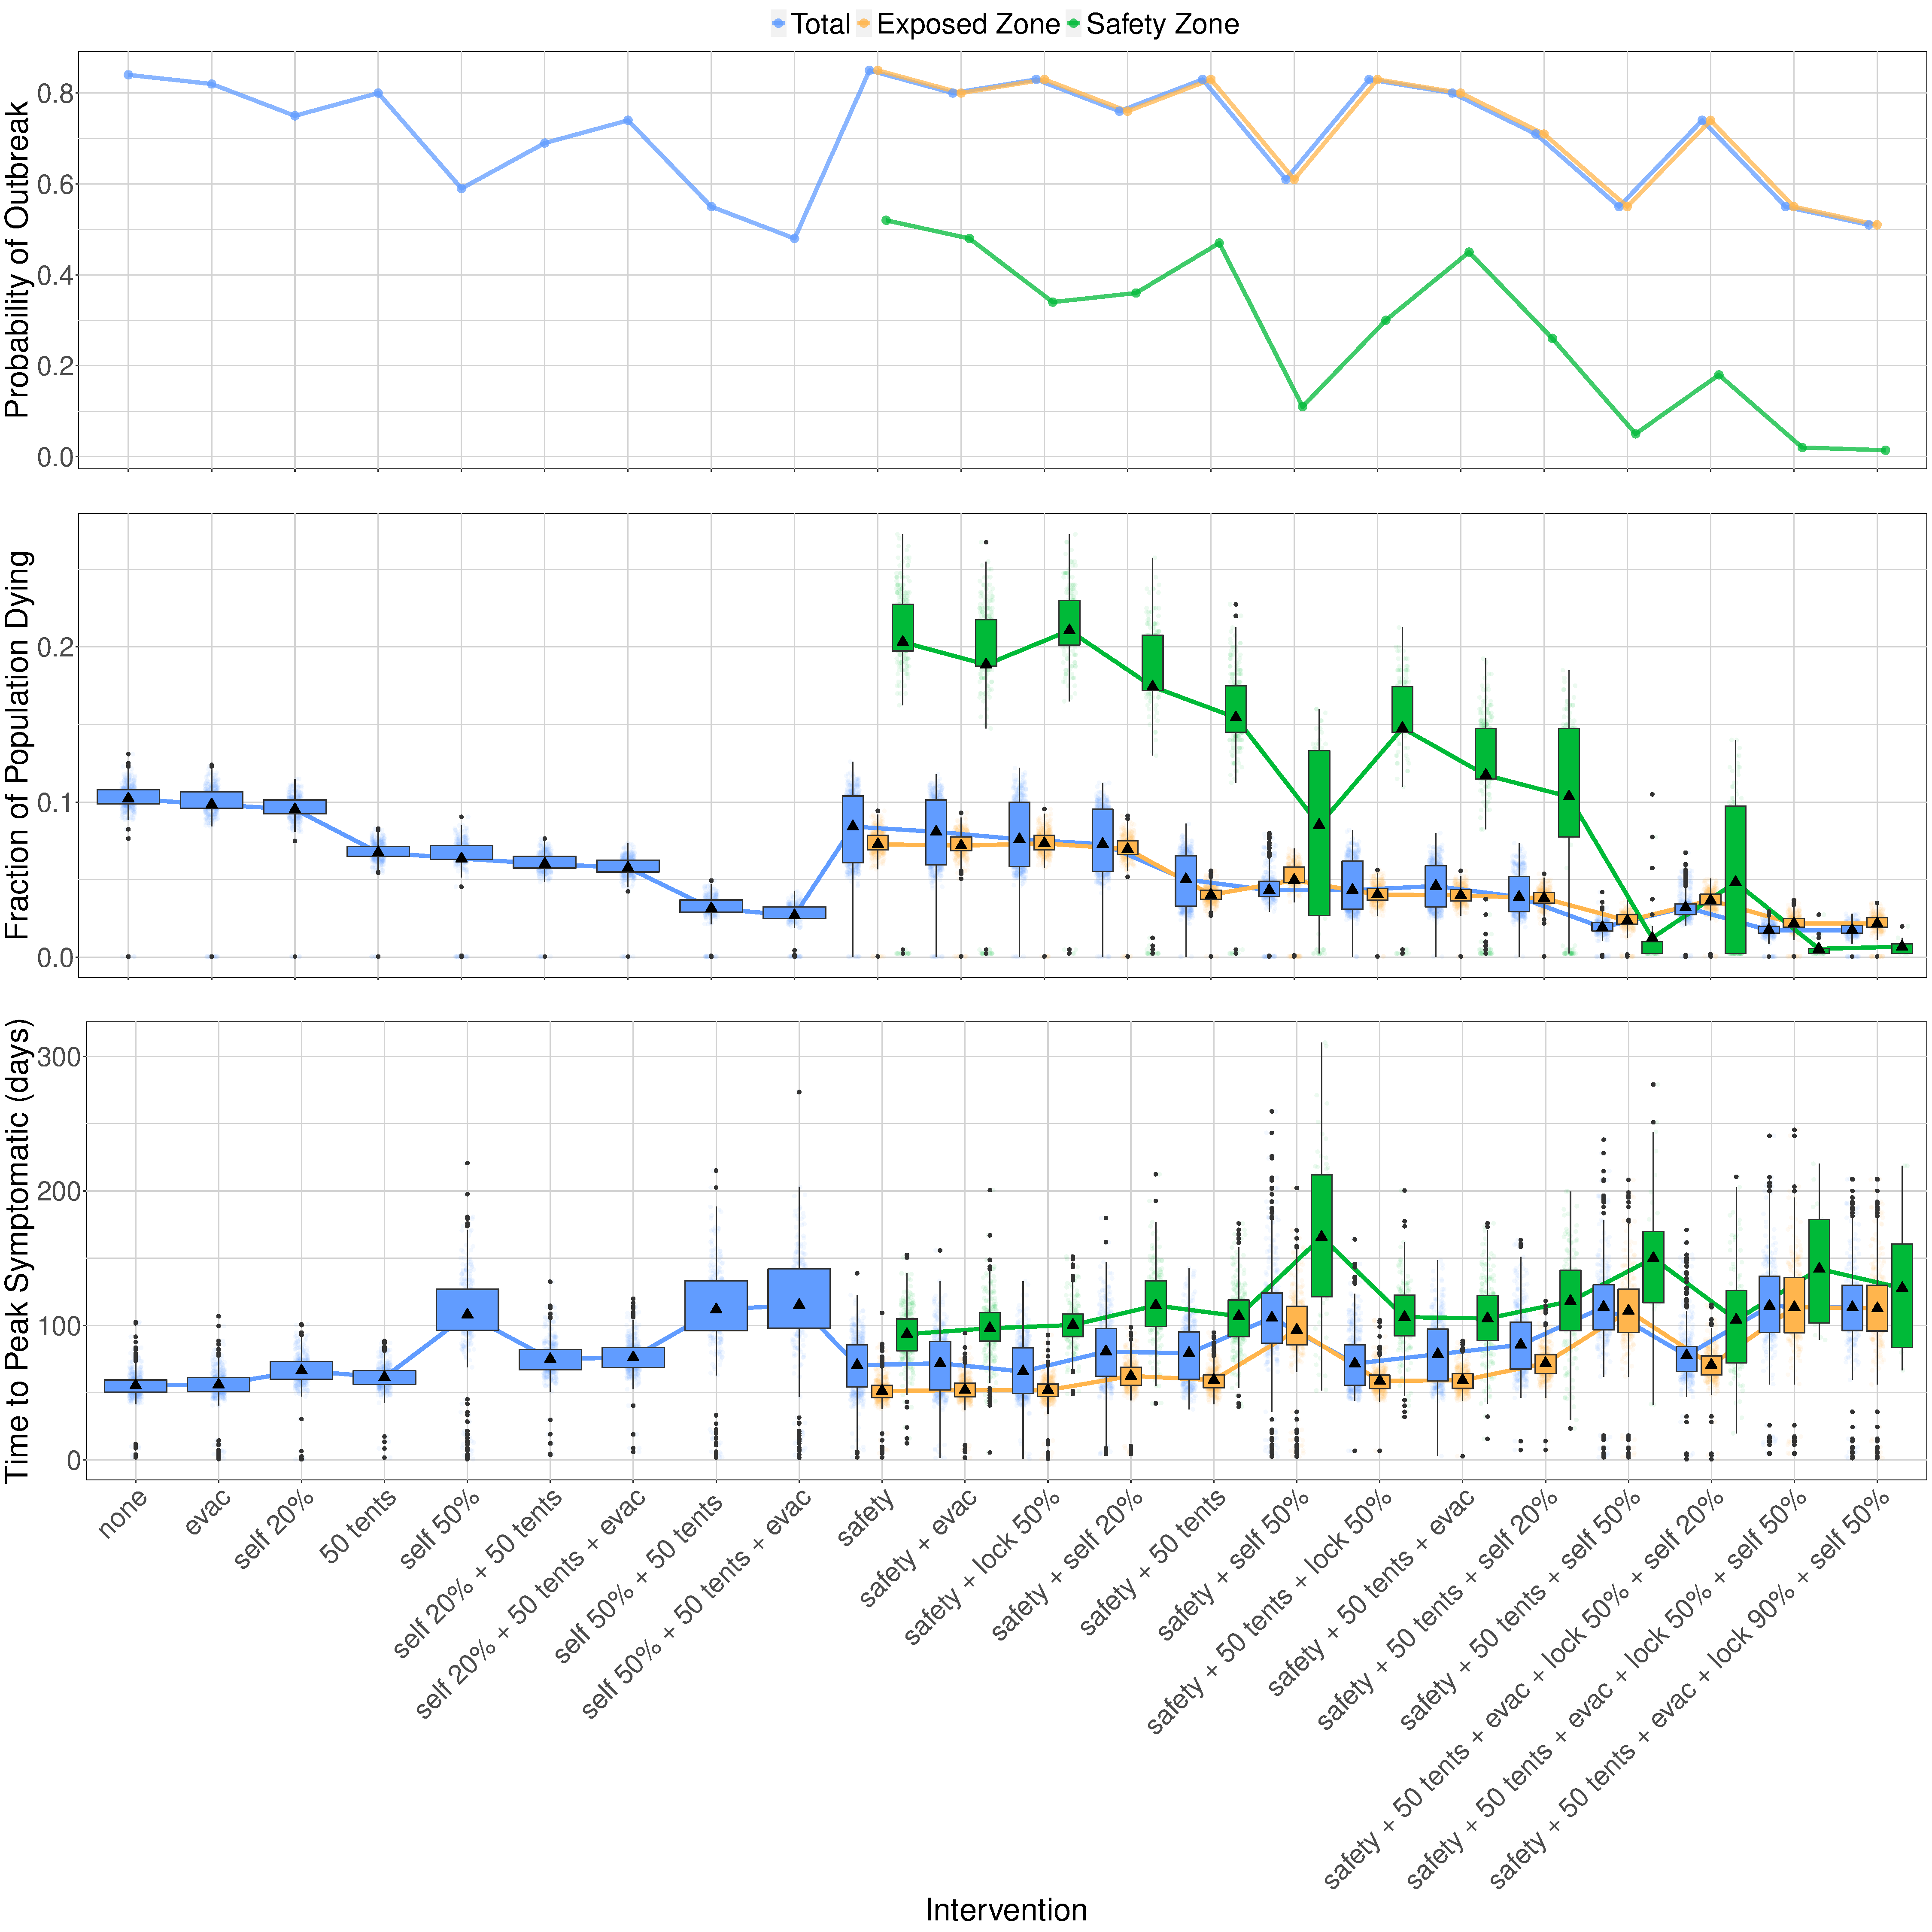
\includegraphics[width=1\textwidth]{figures/Fig3}\\
 
\par\end{centering}
\caption{\label{fig:Panel3} \textbf{Combinations of interventions.} Probability
of an outbreak (top), fraction of the population dying (middle) and
time until peak symptomatic cases (bottom) for different combination
of interventions. Evac = evacuation of severely symptomatic, self
= self-distancing, tents = number of available self-isolation tents,
safety = safety zone, lock = lockdown of the buffer zone. For combinations
of interventions including a safety zone, we distinguish between the
population living in the green zone, in the orange zone and the whole
population.}
\end{figure*}


\section*{Discussion}

In this study, we propose a number of interventions of immediate applicability
to informal settlements. We focused on IDP settlements in NW Syria,
taking into account the interventions' feasibility, cultural acceptance
and their need for low-cost. When confronted with different possible
scenarios, we generally considered the worst-cases, highlighting the
interventions that are most effective in the direst conditions, but
possibly resulting in an overestimate of mortality. Our results align
with previous simulation studies of potential COVID-19 interventions
in similarly densely populated, low-resource settings where informal
settlements are present, such as urban areas of sub-Saharan Africa.
In these settings, social-distancing is demonstrated to be an effective
intervention, and even small changes are estimated to have large effects
on outbreaks \cite{nyabadza2020}, in some cases determining whether
or not already inadequate healthcare systems become overwhelmed \cite{siraj_early_2020}.
Zandvoort et al. show that similar measures to the ones we consider:
self-isolation, physical distancing and ``shielding'' the vulnerable,
may reduce mortality by 60\%-75\% in African cities \cite{vanzandvoort2020}.

Self-distancing proves to be an effective measure in our models as
well; reducing contacts by 50\% has the greatest effect across most
outcomes of interest in any of the interventions we examined. However,
the difficulty of achieving a reduction of this magnitude cannot be
overlooked, especially considering the large proportion of the population
composed of children, a group with an already high contact rate that
may prove difficult to control \cite{noauthor_syrian_nodate}.

We also propose self-isolation using individual tents which can be
located in a dedicated zone or next to the tents of relatives, where
contact with non-isolated individuals is mediated by a buffer zone.
This intervention is effective with even a small number of isolation
tents, as low as 5-10 tents per 1000 camp residents. After conversations
with camp managers, we found that this intervention is more likely
to be accepted in NW Syria than evacuation to community-based isolation
centers. Community-based isolation not only poses cultural challenges;
the capacity required to implement it has hardly been met \cite{UNOCHA_CCTC_numbers}.

One of the key parameters we assessed for the implementation of self-isolation
is the need for carers. In considering one carer per isolated individual,
with daily contact in a buffer zone, once a certain threshold of isolated
cases ($\sim$200 per camp of 2000) is surpassed, the benefits of
isolation begin to be outweighed by an increase in infectivity resulting
from a growing number of exposed carers. This pitfall could be circumvented
through the creation of a more organized, dedicated group of carers,
thus reducing the number of healthy younger adults in contact with
isolated (infectious) individuals.

Much of the success or failure of the safety zone intervention hinges
on the functioning of the buffer zone. The number of inter-zone contacts
per week, the implementation of health checks, and potential lockdowns
all have notable effects. Also important is the portion of the population
that is protected; protecting only the vulnerable may have the most
beneficial effects, but it is precisely these vulnerable individuals,
older adults and people with comorbidities, who may most need family
members to care for them. While safety zone scenarios that allow greater
numbers of family members to accompany their vulnerable relatives
to the green zone may confer greater epidemiological risk, they may
also engender greater well-being and social cohesion.

Although setting up a safety zone sharply reduces the probability
of an outbreak in the population classes with the highest IFRs, thus
reducing the IFR of the entire population, it is possible that our
model may overestimate mortality from an outbreak in the green zone
in the few instances when there is one. Since total numbers of contacts
are conserved in our modelization, individuals do not reduce their
contacts when moved to the green zone, which implies an increase in
the number of contacts between vulnerable individuals. Despite this
increase in contacts, we observed a significant reduction in mortality
in the vulnerable population when the safety zone is implemented.
These results address concerns raised around this type of intervention
from previous experiences with large numbers of fatalities registered
in nursing-homes in developed countries \cite{dahab_covidIDPcontrol_2020}.
While in developed countries nursing home residents have more contacts,
both with other vulnerable people (other nursing home residents) and
healthy adults who live in different households (health aids), than
the elderly who live at home, vulnerable people in our proposed green
zone have the same number of total contacts as they would under normal
conditions, but significantly fewer contacts with healthy adults from
different households.

An instrumental consideration for our models is the fraction of the
population recovered from COVID-19 after a steady state is reached.
Although the duration for which SARS-CoV-2 infection confers immunity
is uncertain, the proportion of the population recovered after an
outbreak should play a role in its protection against future ones.
For every intervention except self-distancing of 50\%, we observed
that the fraction of the population recovered meets or exceeds 75\%.

A key limitation of our approach is that it simulates an outbreak
started by one infectious individual in a single camp with a closed
population. We acknowledge that this approach does not fully capture
the complexities of the NWS region, where IDPs live interspersed throughout
the region in several hundred camps. The dynamics of an outbreak in
the region are undoubtedly influenced by inter-community contacts,
and the dynamics of an outbreak in a single camp by these region-wide
dynamics, as it has been demonstrated in other countries \cite{gatto_spread_2020,arenas2020}.
We expect our results to be robust against changes in the population,
as soon as these changes are relatively small compared to the total
population size in the camp, implying punctual inputs of infected
individuals. This is the expected behaviour in IDPs, which are often
small and located in rural areas, and in which important population
movements, as those observed in large camps, are infrequent.

Other unaccounted for social and cultural dynamics will undeniably
complicate the feasibility of our proposed interventions. Only one
example we have not addressed here is the unlikeliness of children
under 13 self-isolating. Although the number of challenges to implementing
our proposed interventions are potentially endless, the community-based
nature of our approach may help circumvent these challenges much faster
than healthcare-based interventions, which often depend on complex
political decisions and may take years to build the requisite capacity
for an effective response. If the dynamics of the virus are well understood
by local communities and at least some of the interventions we propose
are implemented, the impacts of COVID-19 can be mitigated even in
an environment as challenging as NW Syria.

Given a rapidly changing environment and slow responses of local and
international authorities, empowering local communities themselves
is perhaps the best, if not the only way, to help them avoid the worst
consequences of the pandemic. This not only applies to IDP camps in
NW Syria, but more generally to refugee camps in conflict-torn regions,
and potentially other informal settlements and vulnerable communities
around the world: the low-cost, effective interventions we present
are feasible, needed and urgent.

\section*{Materials and methods}

\subsection*{The model}

The model, adapted for NWS IDP camps is divided into compartments
containing individuals at different possible stages along the disease's
progression \cite{gatto_spread_2020} (see Supplementary Fig. \ref{fig:Diagram}),
and splits the population into classes by age and comorbidity status.
The simulation starts with a completely susceptible population where
one person is exposed to the virus. The disease in exposed individuals
progresses through a preclinical infectious stage, followed by either
a clinical (symptomatic) or subclinical (asymptomatic) infectious
stage, resolving through recovery or death. Additional susceptible
individuals become infected through contact with infectious individuals.
We verified that a steady state was always reached before the end
of each simulation. We did not consider migration, births, nor deaths
due to other causes, since they are small enough in magnitude to not
significantly impact the course of an outbreak, provided additional
conflict does not erupt.

\subsection*{Population structure}

We parameterized the model with data from IDPs in NWS \cite{noauthor_syrian_nodate}.
The population sizes of informal camps are approximately log-normally
distributed, with a mean of of 1212. We simulated camps with populations
of 500, 1000 and 2000 individuals. Since interventions tend to be
less effective in larger camps, the results presented refer to simulations
with 2000 individuals, unless otherwise specified. We considered 3
age groups: children (age 1, 0-12 years old), younger adults (age
2, 13-50 yrs) and older adults (age 3, \textgreater 50 yrs). For
ages 2 and 3, we considered two subclasses comprising healthy individuals
and individuals with comorbidities. The fraction of a simulated camp's
population in each of these 5 classes is shown in Supplementary Table
\ref{tab:PopParams}.

\subsection*{Epidemiological severity assumptions}

We considered a worst-case scenario in which individuals will not
have access to healthcare. We consequently assumed that all critical
cases, those requiring ICU care, would die. However, there is greater
uncertainty about the fate of severe cases, those requiring hospitalization
but not ICU care. We therefore considered a compartment for severe
cases to account for a longer infectious period if they stay in the
camp. This compartment also helped us model some interventions more
realistically, for example by noting that the symptoms of severe cases
are incompatible with self-isolation. To estimate upper and lower
bounds for the outcome variables of our model, we simulated two possible
scenarios for the fate of this compartment: one in which all cases
recover, and another in which all die. In the simulations presented
in the Main Text, we consider the worst-case scenario in which all
of these cases die.

The fractions of symptomatic cases that are severe or critical are
class-specific (parameters $h_{i}$ and $g_{i}$, see Supplementary
Table \ref{tab:PopParams}). We estimated these parameters using data
from developed countries with superior population health \cite{dong2020epidemiological,covid2020preliminary}.
Following previous work \cite{vanzandvoort2020}, we reasoned that
the case severity distributions of NW Syrian adult population classes
would correspond with those of older age groups in developed countries.

\subsection*{Transmissibility assumptions}

We assumed presymptomatic, asymptomatic, symptomatic and hospitalized
individuals were equally infectious. We obtained the duration individuals
spend in each compartment from the literature (see Supplementary Table
\ref{tab:FixedParams}). Inspired by previously proposed models \cite{gatto_spread_2020,vanzandvoort2020},
each individual's contact rate (see Supplementary Table \ref{tab:PopParams})
is class-specific, and was estimated from conversations with camp
managers in NWS. The probability of random interaction with an individual
from each class is proportional to this class' fraction of the population.
The product of these two values is the contact rate between two respective
classes.

The probability of infection from contact with an infectious individual,
$\tau$, was estimated from a Gaussian distribution of the basic reproduction
number, $R_{0}$, with a mean of 4 (99\% CI: 3--5). This distribution
was a compromise between values reported in the literature from regions
with high-density informal settlements: $R_{0}$=2.77 in Abuja and
3.44 in Lagos, Nigeria \cite{oyinlola_empirical_2020}, 3.3 in Buenos
Aires \cite{santos_numerical_2020}, and 5 in Rohingya refugee camps
in Bangladesh \cite{truelove_potential_2020}. The probability distribution
of $\tau$ was estimated by randomly generating a value for $R_{0}$,
and dividing this value by the real part of the main eigenvalue of
the Next Generation Matrix (see Supplementary Material).

\subsection*{Analysis of the interventions}

For each implementation of the interventions, we ran 500 simulations
and compared results between them. The main variables considered are
the fraction of simulations in which at least one death is observed,
a proxy for the probability of an outbreak, the fraction of the population
that dies and the time until the symptomatic population peaks, as
well as the infection fatality rate (IFR) and fraction of the population
that recovers. For consistency, we only considered simulations in
which there was an outbreak when comparing the outcome of a variable
between interventions. We used the Shapiro-Wilk test \cite{shapiro_analysis_1965}
to verify that our results do not exhibit normally distributed residuals,
Kruskal-Wallis test for pairwise comparisons \cite{kruskal_ranks_1952},
and Conover-Iman test for multiple comparisons \cite{conover_multiple_1979}.
The model and all statistical analyses were implemented in R; we used
the package PMCMRplus \cite{pohlert_pmcmr_2020}. All the code and
results are freely available at the url https://github.com/crowdfightcovid19/req-550-Syria.

\section*{Acknowledgements}

This collaboration was organized by crowdfightCOVID19 (www.crowdfightcovid19.org)
upon request from CS. We thank Judith Boumann for valuable contributions.
We thank Peter Ashcroft, Juan Poyatos, Noreen Goldman, Burcu Tepekule
and members of Sebastian Bonhoeffer's and Bryan Grenfell's groups
for useful discussions.

\section*{Declarations}

\subsubsection*{Funding}

ECF's research is supported by Wellcome Trust grant 204833/Z/16/Z.

\subsubsection*{Conflicts of interest/Competing interests}

Alberto Pascual-García is a Board Member of crowdfightCOVID19, an
initiative from the scientific community to put all available resources
at service of the fight against COVID-19. Chamsy Sarkis (co-author)
is a Board Member of the Pax Syriana Foundation, a non-profit organization
set up for social and philanthropic purposes including promoting and
providing support and assistance to civilian aid projects in the fields
of education, health, emergency assistance, psychological assistance
and humanitarian aid for people affected by wars or humanitarian crises.
These organizations had no role in study design, data collection,
data analysis, data interpretation, or writing of the article.

\subsubsection*{Ethics approval}

This study used only publicly available aggregate data and was thus
not subject to ethical review.

\subsubsection*{Consent to participate}

NA

\subsubsection*{Consent for publication}

All authors agreed on publication.

\subsubsection*{Availability of data and material}

All results are available at the url https://github.com/crowdfightcovid19/req-550-Syria

\subsubsection*{Code availability}

All the code is freely available at the url https://github.com/crowdfightcovid19/req-550-Syria

\subsubsection*{Authors' contributions}

All authors contributed to the conceptualization. Design of the methodology:
APG, ECF, JV, JK. Formal analysis: APG, ECF, JK. Code development
APG, ECF, JK. Conducted research: APG, ECF, JV, JK. Validate results:
APG, ECF, JK, JV. Contributed resources: APG, CS, ECF, JK. Data curation:
APG, JK. Visualization: APG, ECF, JK. Writing (original draft) APG,
ECF, JK. All authors contributed to the final version of the manuscript,
and APG supervised the research.

 \bibliographystyle{unsrt}
\bibliography{req550-syria}

\end{document}
